\chapter{Argomento: il sistema Lindenmayer}
{ }\hfill\textbf{Livello:} Avanzato \\


In questo capitolo trarrò informazioni da:
\begin{itemize}
 \item La pagina inglese di Wikipedia circa i sistemi-L: \texttt{http://en.wikipedia.org/wiki/L-System}.
 \item Il libro ``The Algorithmic Beauty of Plants'' scritto da by Przemyslaw Prusinkiewicz e Aristid Lindenmayer.
\end{itemize}

Questa sezione tratterà dei sistemi Lindemayer o sistemi L introdotti e sviluppati nel 1968 dal biologo teoretico Lindenmayer. Un sistema-L è un sistema di regole e simboli utilizzato per modellizare i processi di crescita dello sviluppo delle piante ma anche è anche capace di modellizare la morfologia di una varietà di organismi. Il concetto principale dei sistemi L è il ``regole di sostituzione''. Questa tecnica è utilizzata per sostituire alcune condizioni iniziali utilizzando alcune regole.


\section{definizione formale}
Un sistema-L è una grammatica formale con:
\begin{enumerate}
 \item un \textbf{alfabeto} $V$: l'insieme delle variabili del sistema-L. $V *$ rappresenta l'insieme delle ``parole'' che possiamo generare con qualsiasi simbolo preso dall'alfabeto $V$, e $V +$ l'insieme delle ``parole'' con almeno un simbolo.
 \item Un insieme di valori \textbf{costanti} $S$. Alcuni di questi simboli sono in comune a tutti i sistemi L (in particolare con le tartarughe).
  \item Un \textbf{assioma di partenza} $\omega$ preso da $V +$, è lo stato iniziale.
 \item Un insieme di \textbf{regole} di produzione $P$ dei simboli $V$.
\end{enumerate}
Questo sistema-L è definito come una ennupla (o tupla) $\{V,S,\omega,P\}$.\\

Consideriamo il seguente sistema-L:
\begin{itemize}
	\item Alfabeto : $V = \{A, B\}$
	\item Constanti : $S = \{\emptyset\}$
	\item Assioma iniziale: $\omega = A$
	\item Regole : $\begin{array}{|l|}
	\hline
	A \rightarrow AB \\
	B \rightarrow A \\ 
	\hline
\end{array}
$
\end{itemize}

Le due regole di produzione sono regole di sostituzione. Ad ogni passo il simbolo $A$ è sostituito dalla sequenza $AB$ ed il simbolo $B$ è sostituito da $A$. Ecco le prime iterazioni di questo sistema-Lindemayer:
\begin{center}
	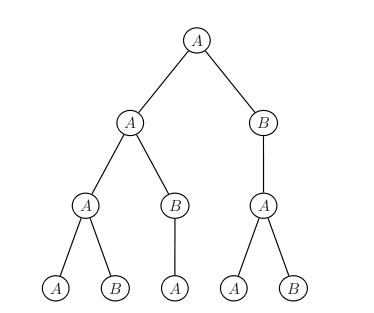
\includegraphics[width=8cm]{pics/linden-arbre.png}
\end{center}
\begin{enumerate}
	\item $A$
	\item $AB$
	\item $ABA$
	\item $ABAAB$
\end{enumerate}
\vspace*{0.2cm}

Ok, ok ma concretamente? Leggiamo la prossima sezione!



\section{L'interpretazione della tartaruga}
Questo primo esempio aiuta a capire cos'è un sistema-L ma ancora non ci fa capire il rapporto con la nostra tartaruga e \logo\textellipsis\\
Qui diventa interessante: tutte le parole che abbiamo costruito non hanno significato. Definiremo per ciascuna lettera della sequenza una azione da eseguire da parte della tartaruga e disegneremo con questo metodo disegni 2D e 3D.


\subsection{Simboli usuali}
\begin{itemize}
 \item $F$ : Av di un passo di una unità ($\in V$)
 \item $+$ : Gira l'angolo a sinistra $\alpha$ $(\in S)$.
 \item $-$ : Gira l'angolo a destra $\alpha$ $(\in S)$.
 \item $\&$ : Beccheggia giù $\alpha$ $(\in S)$.
 \item \textasciicircum : Beccheggia sù $\alpha$ $(\in S)$.
 \item \textbackslash: Rollio a sinistra $\alpha$ $(\in S)$.
 \item $/$: Rollio a destra $\alpha$ $(\in S)$.
 \item $|$: Torna indietro. In \xlogo: \texttt{DX 180}
\end{itemize}
\vspace*{0.2cm}

Per esempio se $\alpha=90$ con un passo di 10 unità abbiamo:
\begin{center}
	\begin{tabular}{|c|c|c|c|c|c|c|c|c|}
		\hline
		Simbolo & $F$ & $+$ & $-$ & $\&$ & \textasciicircum & \textbackslash& $/$ & $|$ \\
		\hline
		Comando \xlogo\ & \texttt{Av 10}&\texttt{SX 90}&\texttt{DX 90}&\texttt{BG 90}&\texttt{BS 90}&\texttt{RSX 90}&\texttt{RDX 90}&\texttt{DX 180}\\
		\hline
	\end{tabular}
\end{center}


\subsection{Il fiocco di neve}
Consideriamo il sistema-L:
\begin{itemize}
 \item [\textbullet] Stato iniziale: $F--F--F--$
 \item [\textbullet] Regole di produzione: $F \rightarrow F+F--F+F$
 \item [\textbullet] Angolo $\alpha=60^{\circ}$, l'unità del passo è divisa per 3 tra ciascuna iterazioni.
\end{itemize}

Prime iterazioni:
\begin{center}
	\begin{minipage}{7.5cm}
		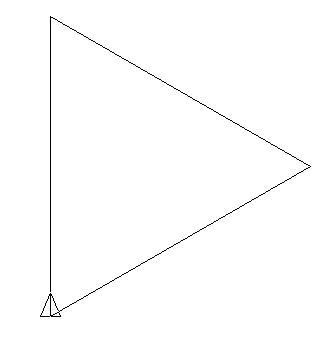
\includegraphics[width=7.5cm]{pics/linden-flocon1.png}
	\end{minipage}
	\begin{minipage}{7.5cm}
		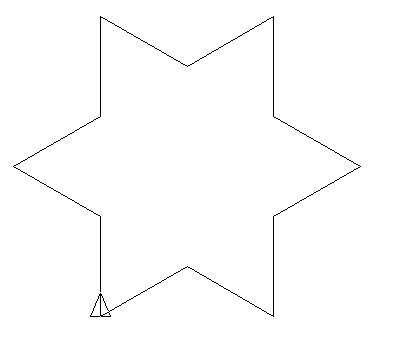
\includegraphics[width=7.5cm]{pics/linden-flocon2.png}
	\end{minipage}\\
	\begin{minipage}{7.5cm}
		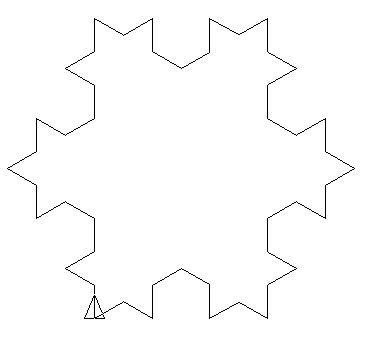
\includegraphics[width=7.5cm]{pics/linden-flocon3.png}
	\end{minipage}
	\begin{minipage}{7.5cm}
		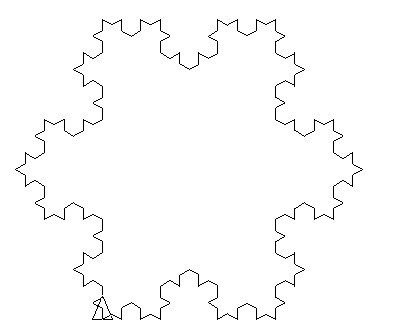
\includegraphics[width=7.5cm]{pics/linden-flocon4.png}
	\end{minipage}
\end{center}

Programma \xlogo:
\begin{lstlisting}[caption="Il fiocco di neve"]
Per FioccoDiNeve :p
	AssegnaVar "unit 300/Potenza 3 :p-1
	Ripeti 3 [f :p-1 DX 120]  
Fine

Per f :p
	Se :p=0 [Av :unit Ferma]
	f :p-1 SX 60 f :p-1 DX 120 f :p-1 SX 60
	f :p-1 
Fine
\end{lstlisting}


\subsection{Curva quadratica di Van Koch}
Dato questo nuovo sistema-L:
\begin{itemize}
 \item[\textbullet] Stato iniziale: $F-F-F-F$
 \item[\textbullet] Regole di produzione: $F\rightarrow F-F+F+FF-F-F+F$
\end{itemize}

Queste sono le prime rappresentazioni utilizzando $\alpha=90$ e dimensionando la dimensione del passo (\texttt{:unita}) in modo che la figura risultante abbia dimensioni costanti.

\begin{center}
\begin{minipage}{7.5cm}
 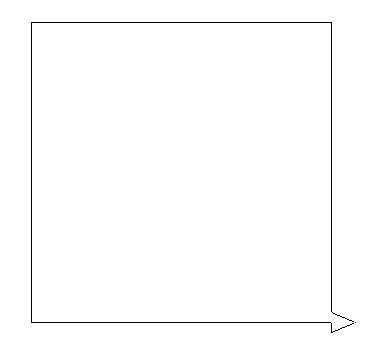
\includegraphics[width=7.5cm]{pics/linden-koch1.png}
\end{minipage}
\begin{minipage}{7.5cm}
 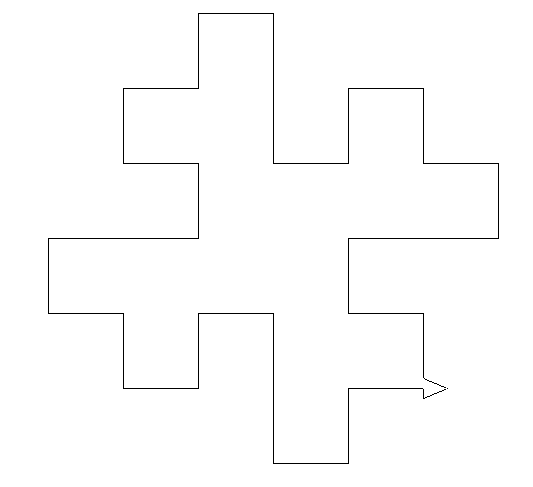
\includegraphics[width=7.5cm]{pics/linden-koch2.png}
\end{minipage}\\
\begin{minipage}{7.5cm}
 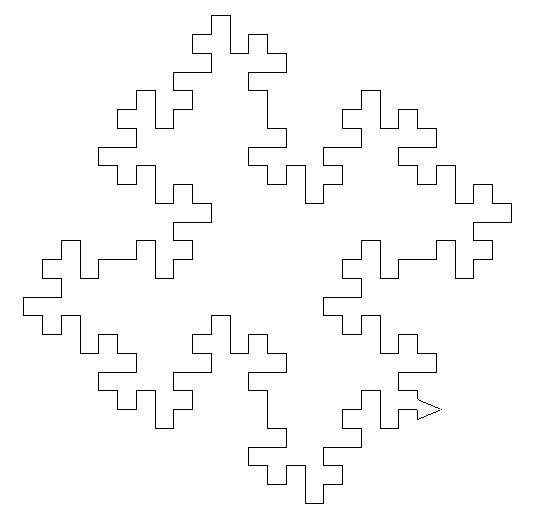
\includegraphics[width=7.5cm]{pics/linden-koch3.png}
\end{minipage}
\begin{minipage}{7.5cm}
 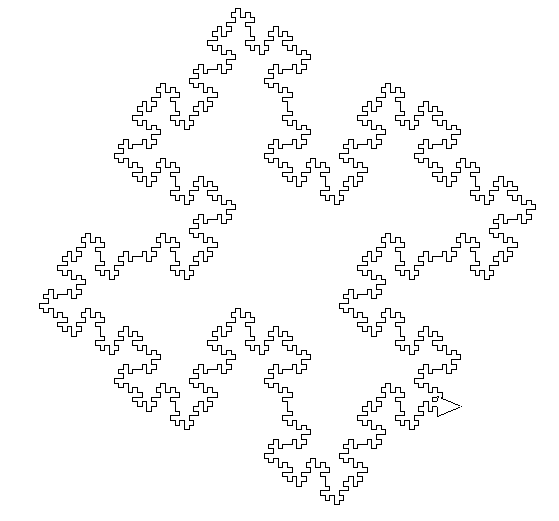
\includegraphics[width=7.5cm]{pics/linden-koch4.png}
\end{minipage}
\end{center}

E' molto semplice creare un programma Logo per generare questi disegni:

\begin{lstlisting}[caption="Curva quadratica di Van Koch"]
# p rappresenta l'ordine
per koch :p
	# la figura finale avra' una dimensione massima di 600x600
	AssegnaVar "unita 300/Potenza 4 :p-1
	Ripeti 3 [f :p-1 SX 90] f :p-1 
fine

# regole di sostituzione
per f :p
	Se :p=0 [Av :unita Ferma]
	f :p-1 SX 90 f :p-1 DX 90 f :p-1 DX 90
	f :p-1 f :p-1 SX 90 f :p-1 SX 90 f :p-1 DX 90 f :p-1
fine
\end{lstlisting}


\subsection{Curva del dragone}
\begin{itemize}
	\item[\textbullet] Stato iniziale: $F$\\
	\item[\textbullet] Regole di produzione:
	$
	\begin{array}{|l|}
		\hline
		A\rightarrow A+B+ \\
		B\rightarrow -A-B \\
		\hline
	\end{array}
	$ 
\end{itemize}

\begin{lstlisting}[caption="Curva del dragone"]
per a :p
	Se :p=0 [Av :unit Ferma]
	a :p-1 SX 90 b :p-1 SX 90
fine

per b :p
	Se :p=0 [Av :unit Ferma]
	DX 90 a :p-1 DX 90 b :p-1
fine

per dragon :p
	AssegnaVar "unit 300/8/ :p  
	a :p
fine
\end{lstlisting}

\begin{center}
	\begin{minipage}{7cm}
		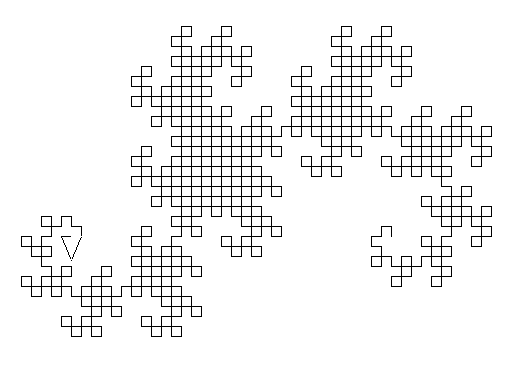
\includegraphics[width=7cm]{pics/linden-dragon10.png}
		\begin{center}
			\texttt{dragon 10}
		\end{center}
	\end{minipage}
	\begin{minipage}{7cm}
		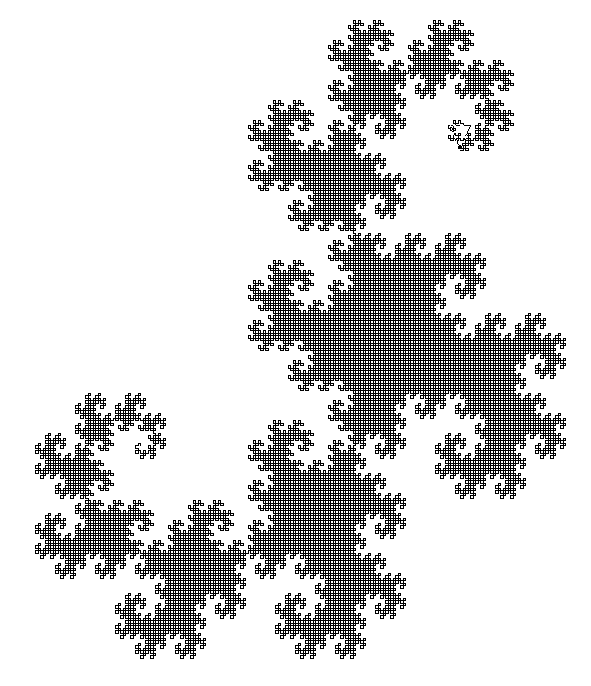
\includegraphics[width=7cm]{pics/linden-dragon15.png}
		\begin{center}
			\texttt{dragon 15}
		\end{center}
	\end{minipage}
\end{center}


\subsection{Curva 3D di Hilbert}
Il seguente esempio genererà una curva 3D di Hilbert. E' una curva singolare perché riempie perfettamente un cubo quando aumentiamo le iterazioni.\\

Questo è il sistema-L da considerare:
\begin{itemize}
	\item Stato iniziale: $A$
	\item Angolo $\alpha=90^{\circ}$, l'unità del passo è divisa per 2 tra due iterazioni.\\
	\item Regole di produzione:
	$
	\begin{array}{|l|}
		\hline
		A\rightarrow B-F+CFC+F-D\&F \textrm{\textrm{\textasciicircum}} D-F+\&\&CFC+F+B// \\
		B\rightarrow A\&F\textrm{\textrm{\textasciicircum}} CFB\textrm{\textasciicircum} F \textrm{\textasciicircum} D\textrm{\textasciicircum} \textrm{\textasciicircum}-F-D\textrm{\textasciicircum}|F\textrm{\textasciicircum} B|FC\textrm{\textasciicircum} F\textrm{\textasciicircum} A// \\
		C\rightarrow|D\textrm{\textasciicircum}|F\textrm{\textasciicircum} B-F+C\textrm{\textasciicircum} F\textrm{\textasciicircum} A\&\&FA\&F\textrm{\textasciicircum} C+F+B\textrm{\textasciicircum} F\textrm{\textasciicircum} D// \\
		D\rightarrow|CFB-F+B|FA\&F\textrm{\textasciicircum} A\&\&FB-F+B|FC// \\
		\hline
	\end{array}
	$
\end{itemize}

\begin{lstlisting}[caption="Curva 3D di Hilbert"]

per hilbert :p
	PS 3D
	AssegnaVar "unit 400/Potenza 2 :p
	FineLinea ImpSP :unit/2
	a :p
	InizioLinea
	VistaPoligono3D
fine

per a :p
	Se :p=0 [Ferma]
	b :p-1 DX 90 Av :unit SX 90  c :p-1 Av :unit c :p-1
	SX 90 Av :unit DX 90 d :p-1 BG 90 Av :unit BS 90 d :p-1
	DX 90 Av :unit SX 90 BG 180 c :p-1 Av :unit c :p-1
	SX 90 Av :unit SX 90 b :p-1 RDX 180
fine

per b :p
	Se :p=0 [Ferma]
	a :p-1 BG 90 Av :unit BS 90 c :p-1 Av :unit b :p-1 BS 90 
	Av :unit BS 90 d :p-1 BS 180 DX 90 Av :unit DX 90 d :p-1 
	BS 90 DX 180 Av :unit BS 90 b :p-1 DX 180 Av :unit c :p-1 
	BS 90 Av :unit BS 90 a :p-1 RDX 180 
fine

per c :p
	Se :p=0 [Ferma]
	DX 180 d :p-1 BS 90 DX 180 Av :unit BS 90 b :p-1 DX 90
	Av :unit SX 90 c :p-1 BS 90 Av :unit BS 90 a :p-1 BG 180
 	Av :unit a :p-1 BG 90 Av :unit BS 90 c :p-1 SX 90 Av :unit 
	SX 90 b :p-1 BS 90 Av :unit BS 90 d :p-1 RDX 180 
fine

per d :p
	Se :p=0 [Ferma]
	DX 180 c :p-1 Av :unit b :p-1 DX 90 Av :unit SX 90 b :p-1 DX 180
	Av :unit a :p-1 BG 90 Av :unit BS 90 a :p-1 BG 180 Av :unit
	b :p-1 DX 90 Av :unit SX 90 b :p-1 DX 180 Av :unit c :p-1 RDX 180
fine
\end{lstlisting}

E le prime iterazioni:
\begin{center}
	\begin{minipage}{7cm}
		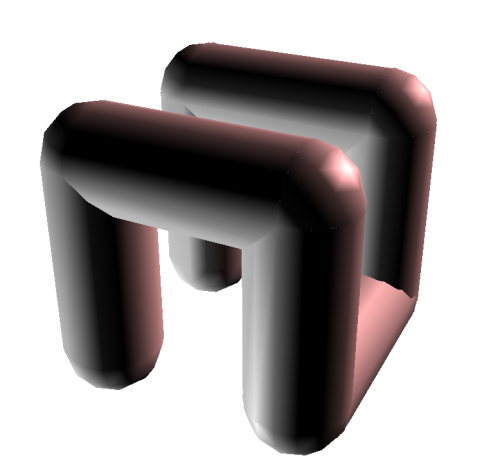
\includegraphics[width=7cm]{pics/linden-hilbert1.png}
	\end{minipage}
	\begin{minipage}{7cm}
		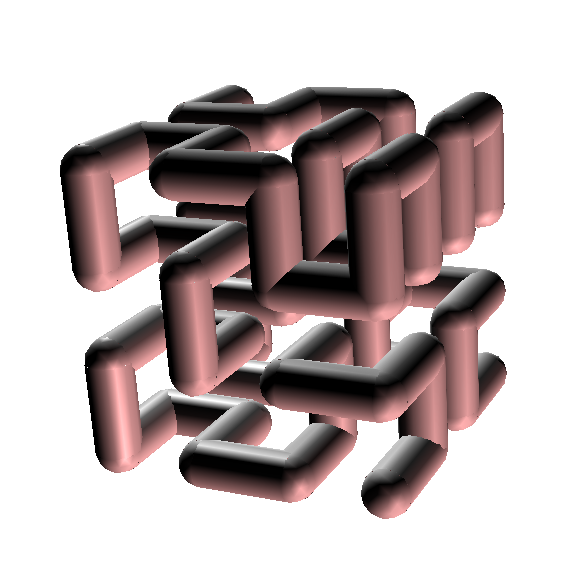
\includegraphics[width=7.5cm]{pics/linden-hilbert2.png}
	\end{minipage}\\
	\begin{minipage}{7cm}
		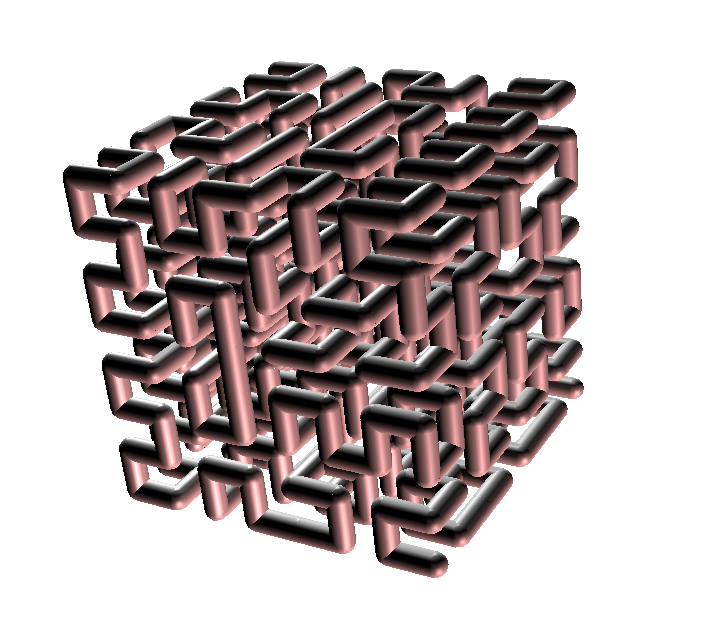
\includegraphics[width=7cm]{pics/linden-hilbert3.png}
	\end{minipage}
	\begin{minipage}{7cm}
		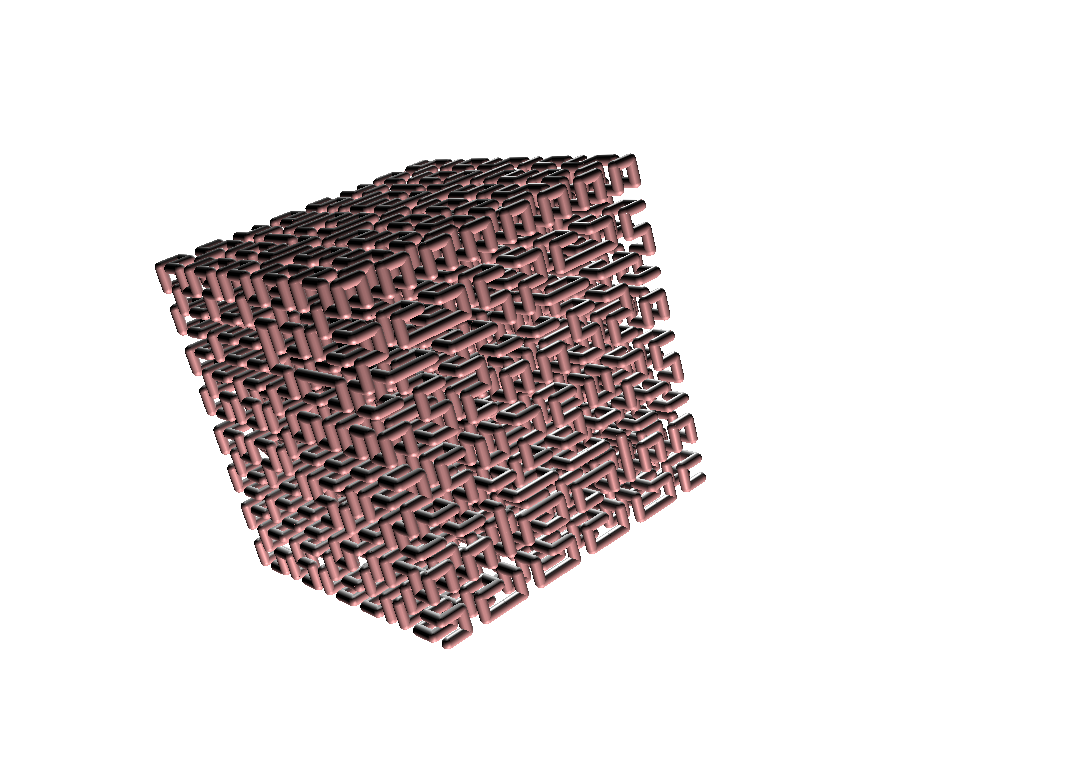
\includegraphics[width=9cm]{pics/linden-hilbert4.png}
	\end{minipage}
\end{center}
Bello, non è vero?